\begin{figure}[H]
	\centering
	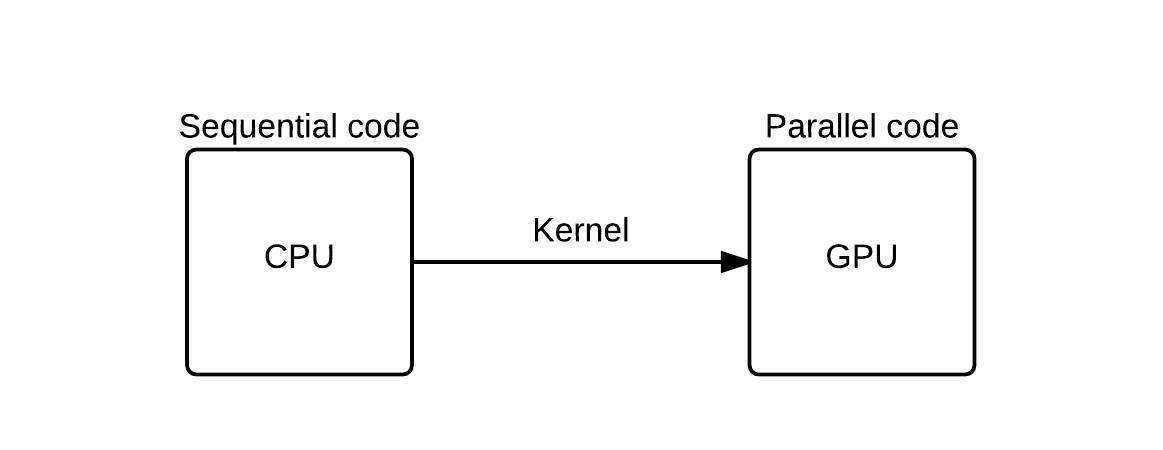
\includegraphics[width=\textwidth]{system_overview/diagrams/programming_model_cpu_gpu.png}
	\caption{Relationship between CPU and GPU code.}
	\label{fig:programming_model_cpu_gpu}
\end{figure}
Programming for Demolicious will seem familiar for readers with programming experience from technology like CUDA or OpenCL. 
Many applications can be divided into sequential and parallel parts, where each part can benefit from different execution models. \todo{Is this a word<Execution model>?}
On the Demolicious system, the sequential parts of a program will be run by the CPU, and the parallel parts can be performed by the GPU through kernels.
A kernel is a simple program meant to be executed by multiple threads.
The kernels are usually uploaded to the GPU at the start of the program, and then executed when requested by the CPU.
This architecture is well suited for highly parallel tasks such as graphics.

\subsection{Kernels}
Kernels are meant to be executed in very high volumes on the GPU.
Each thread in the kernel is assigned a unique thread id.
The thread id can be used to vary the output from kernels, 
by using it to compute memory addresses, selecting color, or other properties.
To keep the architecture simple, kernels support a fairly limited instruction set.
Most notably, the control flow in kernels is linear, meaning they cannot do any branches or jumps.
Although the kernels don't support diverging control flow,
it's simulated by supporting conditional execution through masking.
Each of the instructions in the instruction set can be executed conditionally by prefixing them with \textit{?}.
\begin{figure}[H]
	\centering
	\begin{verbatim}
	  add $1, $1, $2 ; This instruction will be executed unconditionally.
	? add $1, $0, $0 ; This instruction will be executed conditionally.
	\end{verbatim}
	\caption{Conditionally zeroing a register.}
	\label{fig:conditional_execution}
\end{figure}
Whether a conditional instruction is executed, is controlled by a dedicated masking register. 

\subsection{Memories}

\begin{figure}[H]
	\centering
	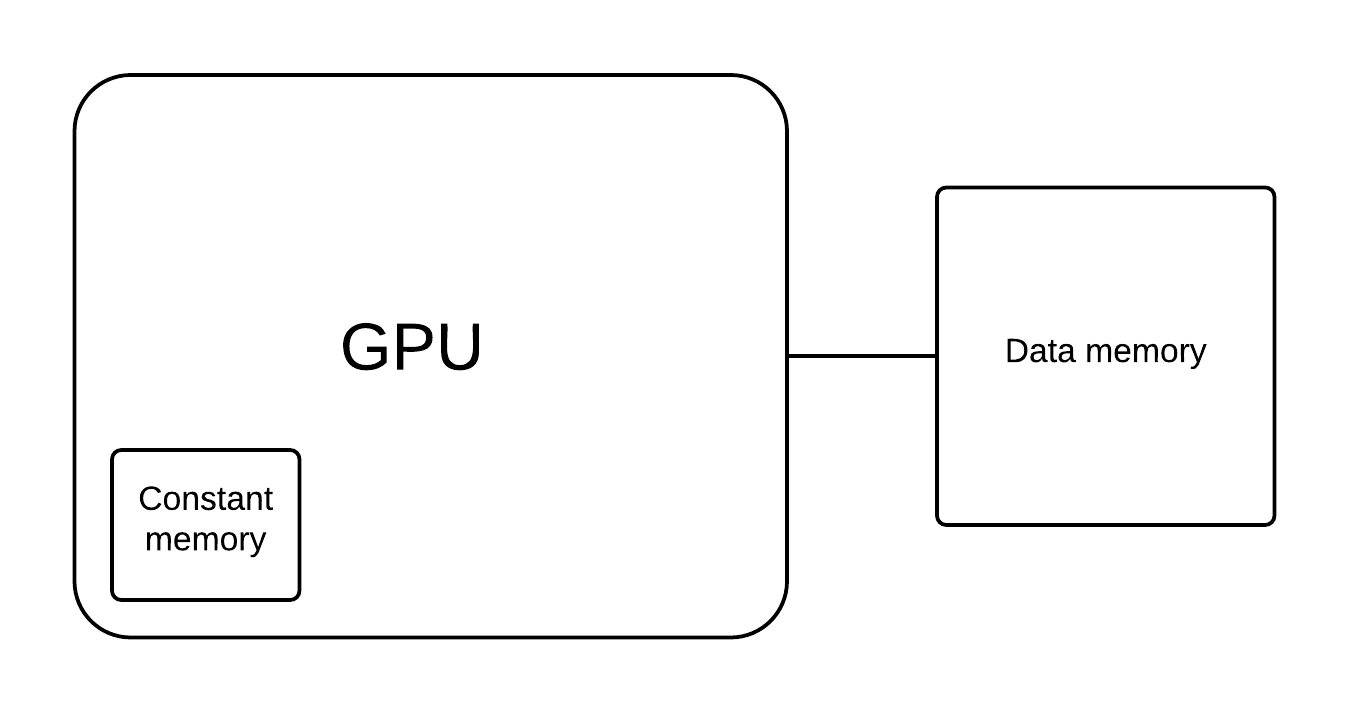
\includegraphics[width=\textwidth]{system_overview/diagrams/memory_overview.png}
	\caption{Overview of GPU memory architecture.}
	\label{fig:memory_overview}
\end{figure}

The Demolicious system contains two memories (Figure \ref{fig:memory_overview}), which the programmer can use.
The data memory is large, but has relatively high latency and low throughput.
Constant memory is small, but very fast.
It will typically be used for kernel parameters,
which will allow kernels to be re-used with varying output.
